\section{基础知识}

\begin{figure}[H]
\centering
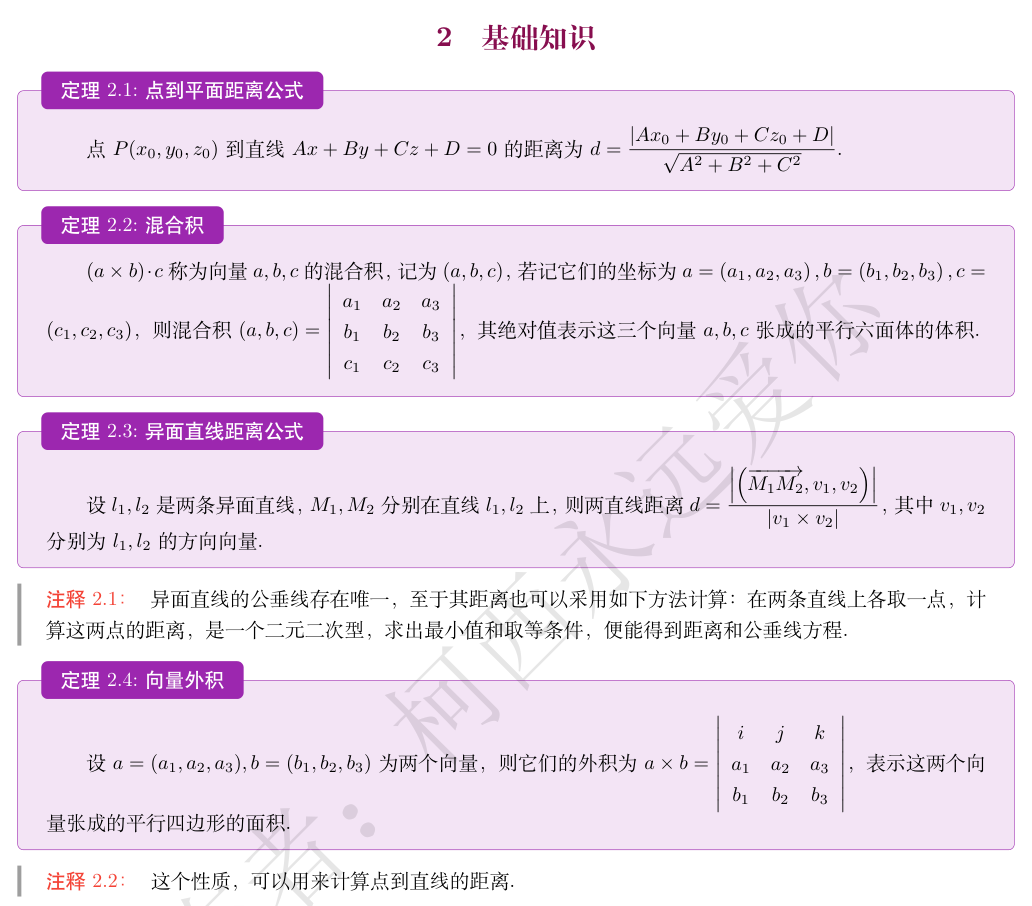
\includegraphics[width=\textwidth]{数学类解析几何-2025040420.png}
% \caption{}
\label{}
\end{figure}

\subsection{判断曲面类型}

见《解析几何》·吕林根·第四版

二次曲面的一般方程为
\[
a_{11}x^2+a_{22}y^2+a_{33}z^2+2a_{12}xy+2a_{13}xz+2a_{23}yz+2a_{14}x+2a_{24}y+2a_{34}z+a_{44}=0
\]
适当选取坐标系,二次曲面的方程总可以化为下列五个方程之一:

\begin{enumerate}
	\item $a_{11}x^2+a_{22}y^2+a_{33}z^2+a_{44}=0,a_{11}a_{22}a_{33}\neq0$.
	\item $a_{11}x^2+a_{22}y^2+2a_{34}z=0,a_{11}a_{22}a_{34}\neq0$.
	\item $a_{11}x^2+a_{22}y^2+a_{44}=0,a_{11}a_{22}\neq0$.
	\item $a_{11}x^2+2a_{24}y=0,a_{11}a_{24}\neq0$.
	\item $a_{11}x^2+a_{44}=0,a_{11}\neq0$.
\end{enumerate}

通过适当选取坐标系,二次曲面的方程总可以化成以下十七种形式之一:

\subsubsection{常见的二次曲面}

椭球面
\[
\frac{x^2}{a^2}+\frac{y^2}{b^2}+\frac{z^2}{c^2}=1
\]
单叶双曲面
\[
\frac{x^2}{a^2}+\frac{y^2}{b^2}-\frac{z^2}{c^2}=1
\]
双叶双曲面
\[
\frac{x^2}{a^2}+\frac{y^2}{b^2}-\frac{z^2}{c^2}=-1
\]
二次锥面
\[
\frac{x^2}{a^2}+\frac{y^2}{b^2}-\frac{z^2}{c^2}=0
\]
椭圆抛物面
\[
\frac{x^2}{a^2}+\frac{y^2}{b^2}=2z
\]
双曲抛物面\sidenote{也叫马鞍面}
\[
\frac{x^2}{a^2}-\frac{y^2}{b^2}=2z
\]
椭圆柱面
\[
\frac{x^2}{a^2}+\frac{y^2}{b^2}=1
\]
双曲柱面
\[
\frac{x^2}{a^2}-\frac{y^2}{b^2}=1
\]
抛物柱面
\[
x^2=2py
\]
\subsubsection{其余的不常见的二次曲面}

虚椭球面
\[
\frac{x^2}{a^2}+\frac{y^2}{b^2}+\frac{z^2}{c^2}=-1
\]
点(虚母线二次锥面)
\[
\frac{x^2}{a^2}+\frac{y^2}{b^2}+\frac{z^2}{c^2}=0
\]
虚椭圆柱面
\[
\frac{x^2}{a^2}+\frac{y^2}{b^2}=-1
\]
交于一条实直线的一对共轭虚平面
\[
\frac{x^2}{a^2}+\frac{y^2}{b^2}=0
\]
一对相交平面
\[
\frac{x^2}{a^2}-\frac{y^2}{b^2}=0
\]
一对平行平面
\[
x^2=a^2
\]
一对平行的共轭虚平面
\[
x^2=-a^2
\]
一对重合平面
\[
x^2=0
\]
\subsection{直母线}

\begin{figure}[H]
\centering
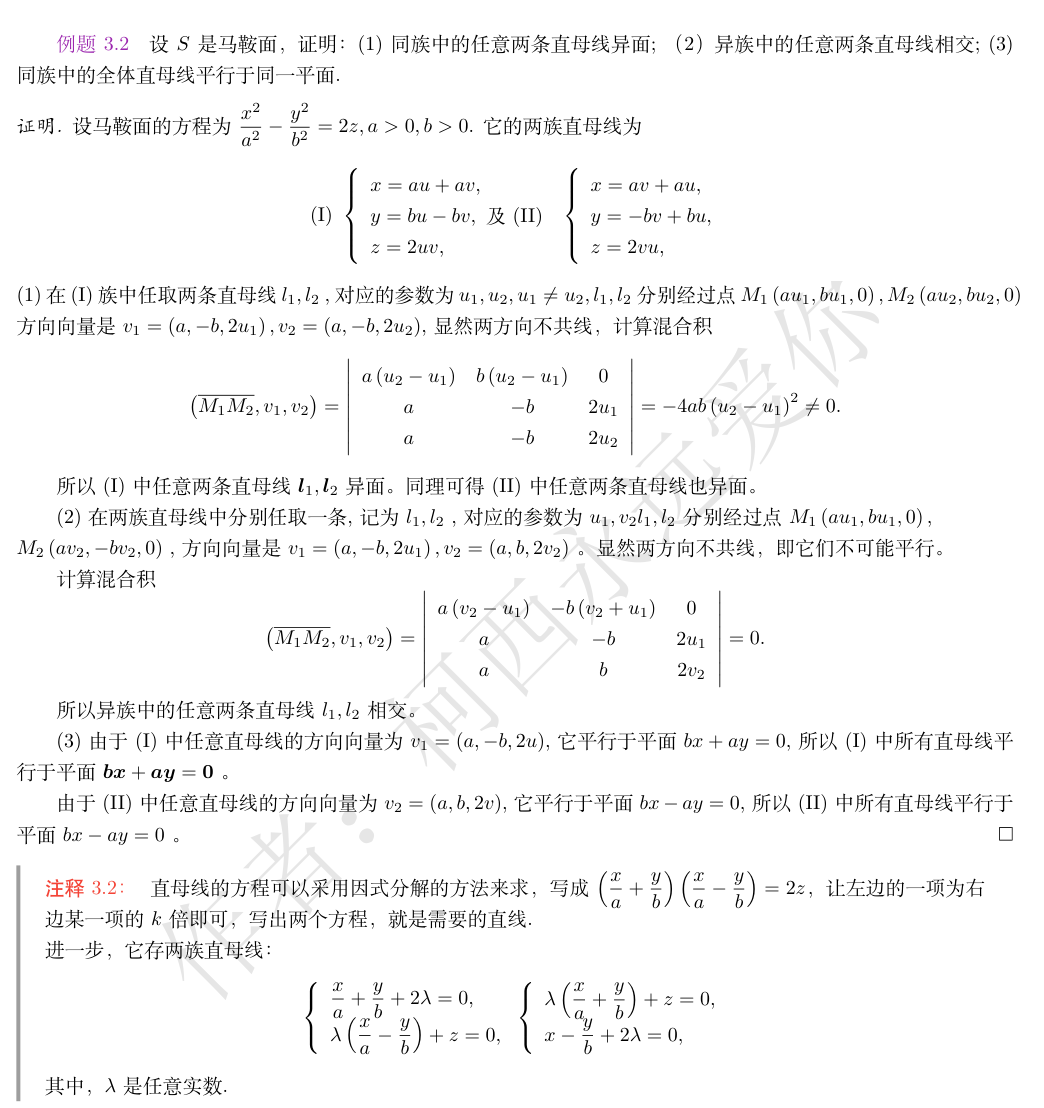
\includegraphics[width=\textwidth]{数学类解析几何-2025040422.png}
% \caption{}
\label{}
\end{figure}

\subsection{与二次曲面交线为圆的平面}

\begin{figure}[H]
\centering
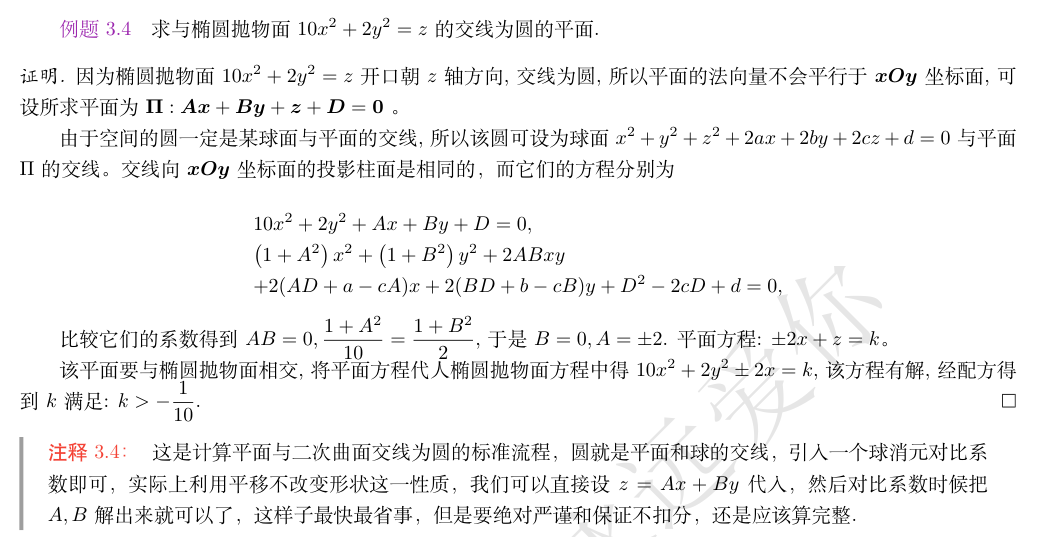
\includegraphics[width=\textwidth]{1-数学类解析几何-2025040422.png}
% \caption{}
\label{}
\end{figure}
